\usetikzlibrary{arrows}
\pagestyle{empty}
\begin{document}
\begin{center}
    \noindent
    Созданный с помощью Geogebra:

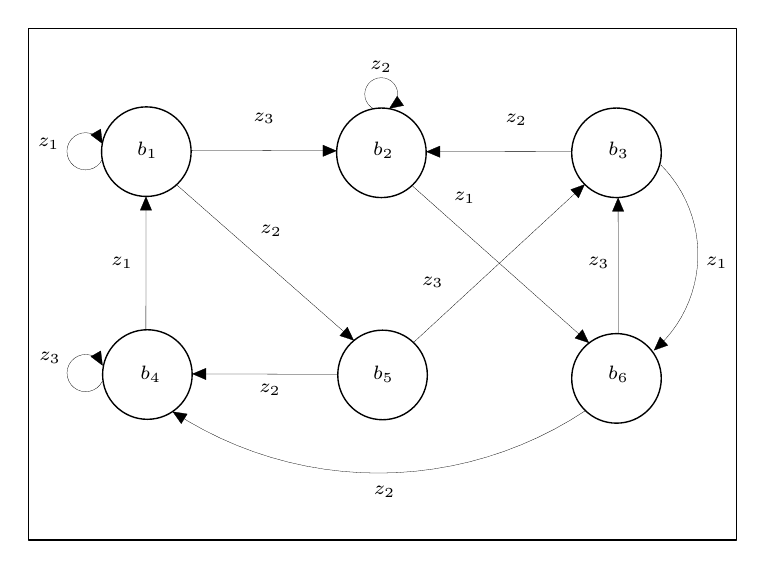
\begin{tikzpicture}[line cap=round,line join=round,>=triangle 45,x=1cm,y=1cm]

\draw (-4.5,-3.5) rectangle (4.5,3);
\draw [line width=0.5pt] (2.9708949242827054,-1.4470035613714107) circle (0.5687031205152061cm);
\draw [line width=0.5pt] (2.970894924282706,1.4178984856541166) circle (0.5687031205152331cm);
\draw [line width=0.5pt] (0,-1.4033459477954695) circle (0.568703120515207cm);
\draw [line width=0.5pt] (-0.014552537858647102,1.4178984856541166) circle (0.5687031205152336cm);
\draw [line width=0.5pt] (-3,1.4324510235127637) circle (0.5687031205152334cm);
\draw [line width=0.5pt] (-2.986664196004032,-1.3980664321823293) circle (0.5687031205152326cm);

\draw [->,line width=0.1pt] (-2.4315268473218885,1.448622417020211) -- (-0.5827129394473904,1.4427379170139971);
\draw [->,line width=0.1pt] (2.4024039088770754,1.4334292514703608) -- (0.5539799587817273,1.4318282935360354);
\draw [->,line width=0.1pt] (0.3735270838599657,1.0021853075005935) -- (2.6224007236130737,-0.9975872383663738);
\draw [->,line width=0.1pt] (0.39229483108621066,-0.991608161350291) -- (2.567903158183671,1.0166244200329453);
\draw [->,line width=0.1pt] (2.9931126707395,-0.8787346012599907) -- (2.9915469281428897,0.8495704694343259);
\draw [->,line width=0.1pt] (-3.0058922975493934,-0.8296884598833278) -- (-3.004666132735822,0.8637670458159625);
\draw [->,line width=0.1pt] (-2.616267564247627,1.012721757157277) -- (-0.3634898625164298,-0.9659692690258752);
\draw [->,line width=0.1pt] (-0.5686423133586304,-1.3950297742836089) -- (-2.4180158195747135,-1.390175724478738);

\draw [<-, shift={(2.3967395313364595,0.126754489390692)},line width=0.1pt]  plot[domain=-0.8603882048439315:0.7863479730960713,variable=\t]({1*1.608263296528255*cos(\t r)+0*1.608263296528255*sin(\t r)},{0*1.608263296528255*cos(\t r)+1*1.608263296528255*sin(\t r)});
\draw [<-, shift={(-0.05337578460024872,2.1105180961775076)},line width=0.1pt]  plot[domain=4.131218338684883:5.297807224399998,variable=\t]({1*4.760402030350322*cos(\t r)+0*4.760402030350322*sin(\t r)},{0*4.760402030350322*cos(\t r)+1*4.760402030350322*sin(\t r)});
\draw [<-, shift={(-3.7719801814250915,1.4369936551945872)},line width=0.1pt]  plot[domain=0.4110144652240396:5.832176174009245,variable=\t]({1*0.2362826572245055*cos(\t r)+0*0.2362826572245055*sin(\t r)},{0*0.2362826572245055*cos(\t r)+1*0.2362826572245055*sin(\t r)});
\draw [<-, shift={(-3.770945616120117,-1.3795850640439742)},line width=0.1pt]  plot[domain=0.41101446522403806:5.832176174009247,variable=\t]({1*0.23628265722450625*cos(\t r)+0*0.23628265722450625*sin(\t r)},{0*0.23628265722450625*cos(\t r)+1*0.23628265722450625*sin(\t r)});
\draw [<-, shift={(-0.016668102767723764,2.1623099343841052)},line width=0.1pt]  plot[domain=-1.0745935833821765:4.2218700808118665,variable=\t]({1*0.20939539267107515*cos(\t r)+0*0.20939539267107515*sin(\t r)},{0*0.20939539267107515*cos(\t r)+1*0.20939539267107515*sin(\t r)});

\begin{scriptsize}
\draw[color=black] (-2.9866641960040314,1.4524800977696472) node {$b_1$};
\draw[color=black] (0.011158602877274187,1.4524800977696472) node {$b_2$};
\draw[color=black] (2.9980864774758747,1.4524800977696472) node {$b_3$};
\draw[color=black] (-2.94487434743862,-1.395817322525182) node {$b_4$};
\draw[color=black] (0.011158602877274187,-1.395817322525182) node {$b_5$};
\draw[color=black] (2.994428863899933,-1.395817322525182) node {$b_6$};
\draw[color=black] (4.245947119743585,0.02267377404629129) node {$z_1$};
\draw[color=black] (1.0443887908412195,0.8503006669786457) node {$z_1$};
\draw[color=black] (-3.306820028894268,0.02267377404629129) node {$z_1$};
\draw[color=black] (-4.238182451847684,1.5342699463350589) node {$z_1$};
\draw[color=black] (0.025711140735921303,-2.8859660326725967) node {$z_2$};
\draw[color=black] (1.6992529944803396,1.8398732413666476) node {$z_2$};
\draw[color=black] (-1.4149901072701432,0.4282770690778801) node {$z_2$};
\draw[color=black] (-1.4295426451287903,-1.5926579282635355) node {$z_2$};
\draw[color=black] (-0.017946472840020045,2.5130255128854732) node {$z_2$};
\draw[color=black] (-1.5023053344220259,1.8544257792252947) node {$z_3$};
\draw[color=black] (0.6369177307991002,-0.22658713456123883) node {$z_3$};
\draw[color=black] (2.7470357203029323,0.02267377404629129) node {$z_3$};
\draw[color=black] (-4.223629913989036,-1.1870546332319467) node {$z_3$};

\end{scriptsize}
\end{tikzpicture}
\end{center}
\end{document}
